%\documentclass[12pt,preprint]{aastex6}
\documentclass[12pt]{article}

\bibliographystyle{aasjournal}

\usepackage{aas_macros} % need this because not using aastex or emulateapj
\usepackage{graphicx}
\usepackage[suffix=]{epstopdf}
\usepackage{natbib}
\usepackage{amsmath}
%\usepackage{url}
\usepackage{xspace}
\usepackage{fullpage}

%    Make Scientific Notation
\providecommand{\e}[1]{\ensuremath{\times 10^{#1}}}

% make the word Kepler italicized
\newcommand{\Kepler}{\textsl{Kepler}\xspace}

\begin{document}
%%%%%%%%%%%%%%%%%%%%%%

%Measuring Stellar Rotation with K2

\title{Scientific/Technical/Management}
\date{}

\maketitle


% shrink up the space between the "title" and first section heading
\vspace{-1in}

%%%%%%%%%%%%%%%%%%%
\section{Introduction}
%\noindent
Stellar rotation periods are are the most promising tool for constraining the ages of field stars.



%%%%%%%%%%%%%%%%%%%
\section{Project Description}

%%%%%%%%%
\subsection{Mining K2 Data for Rotation Periods}


%%%%%%%%%
\subsection{Age-Dating Field Stars with K2}


%%%%%%%%%
\subsection{Solving the Period Bimodality Mystery}

\begin{figure}[!th]
\centering
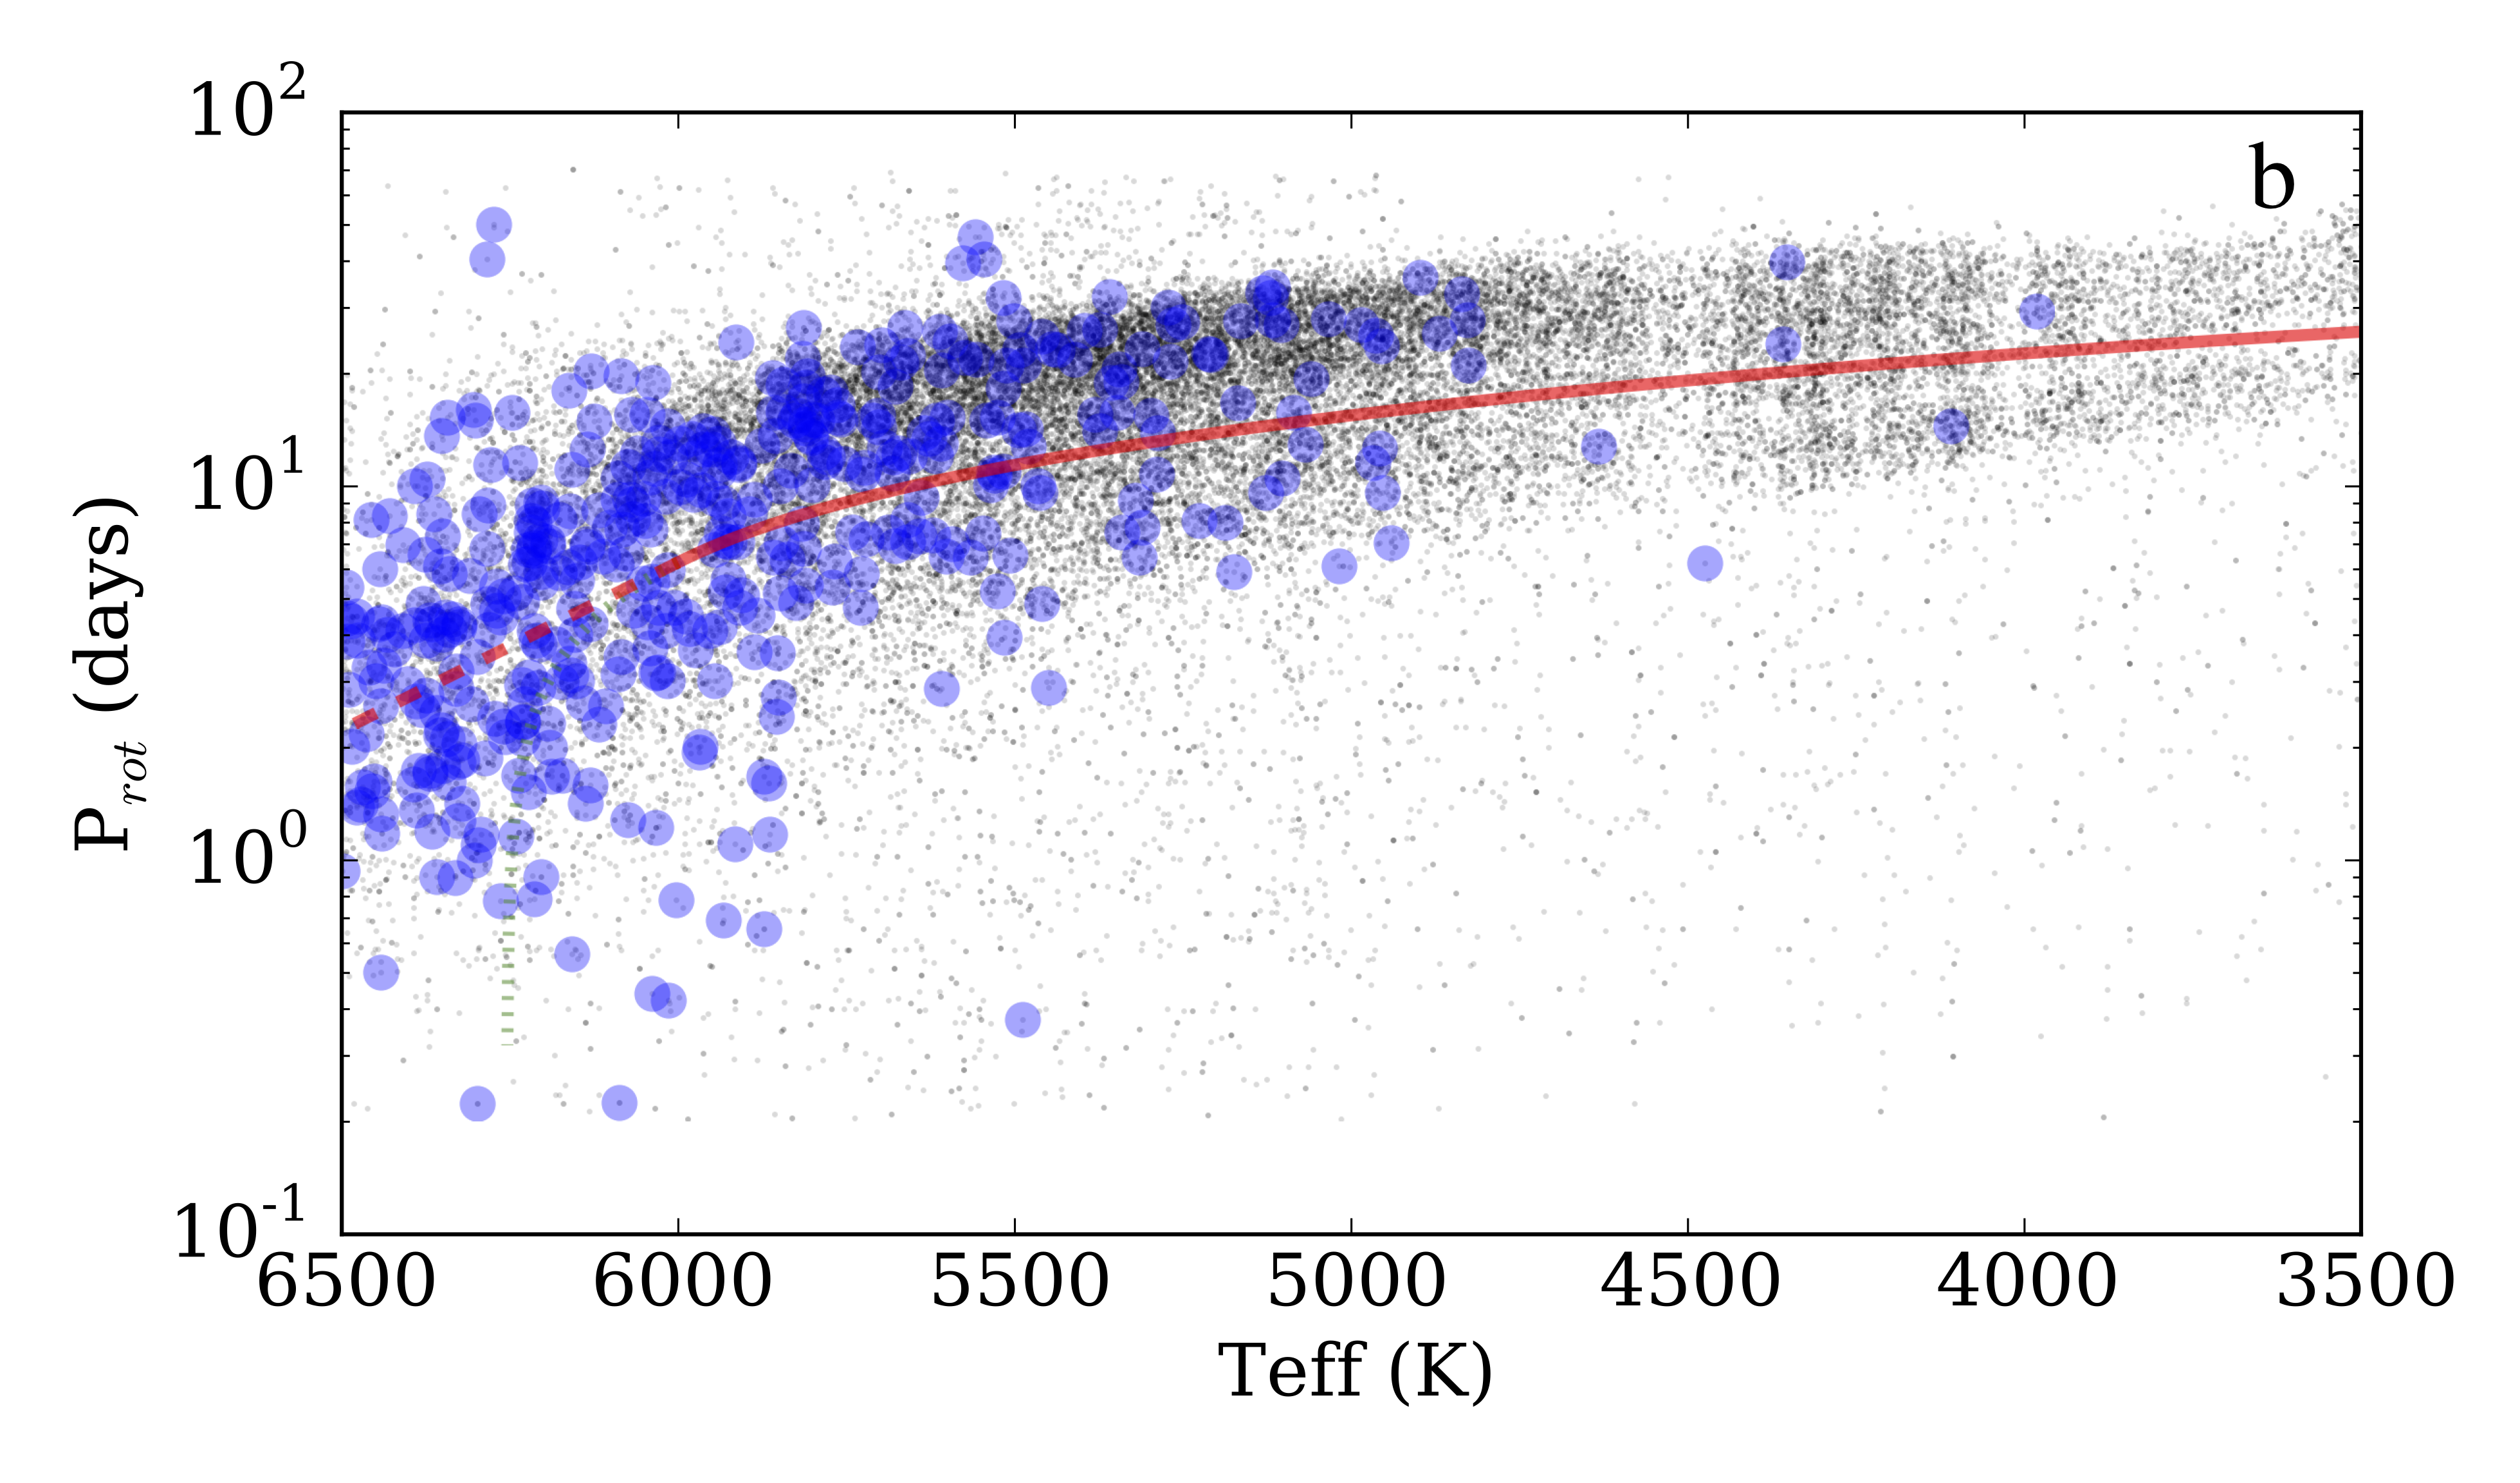
\includegraphics[width=4.5in]{davenport2016_fig3}
\caption{figure 3 from \citet{davenport2017}, showing bimodality in rotation periods from \Kepler}
\label{fig:bimodal}
\end{figure}






%%%%%%%%%%%%%%%%%%%
\section{Plan of Work}

%%%%%%%%%
\subsection{Measuring Rotation Using TOOL}


\begin{figure}[!th]
\centering
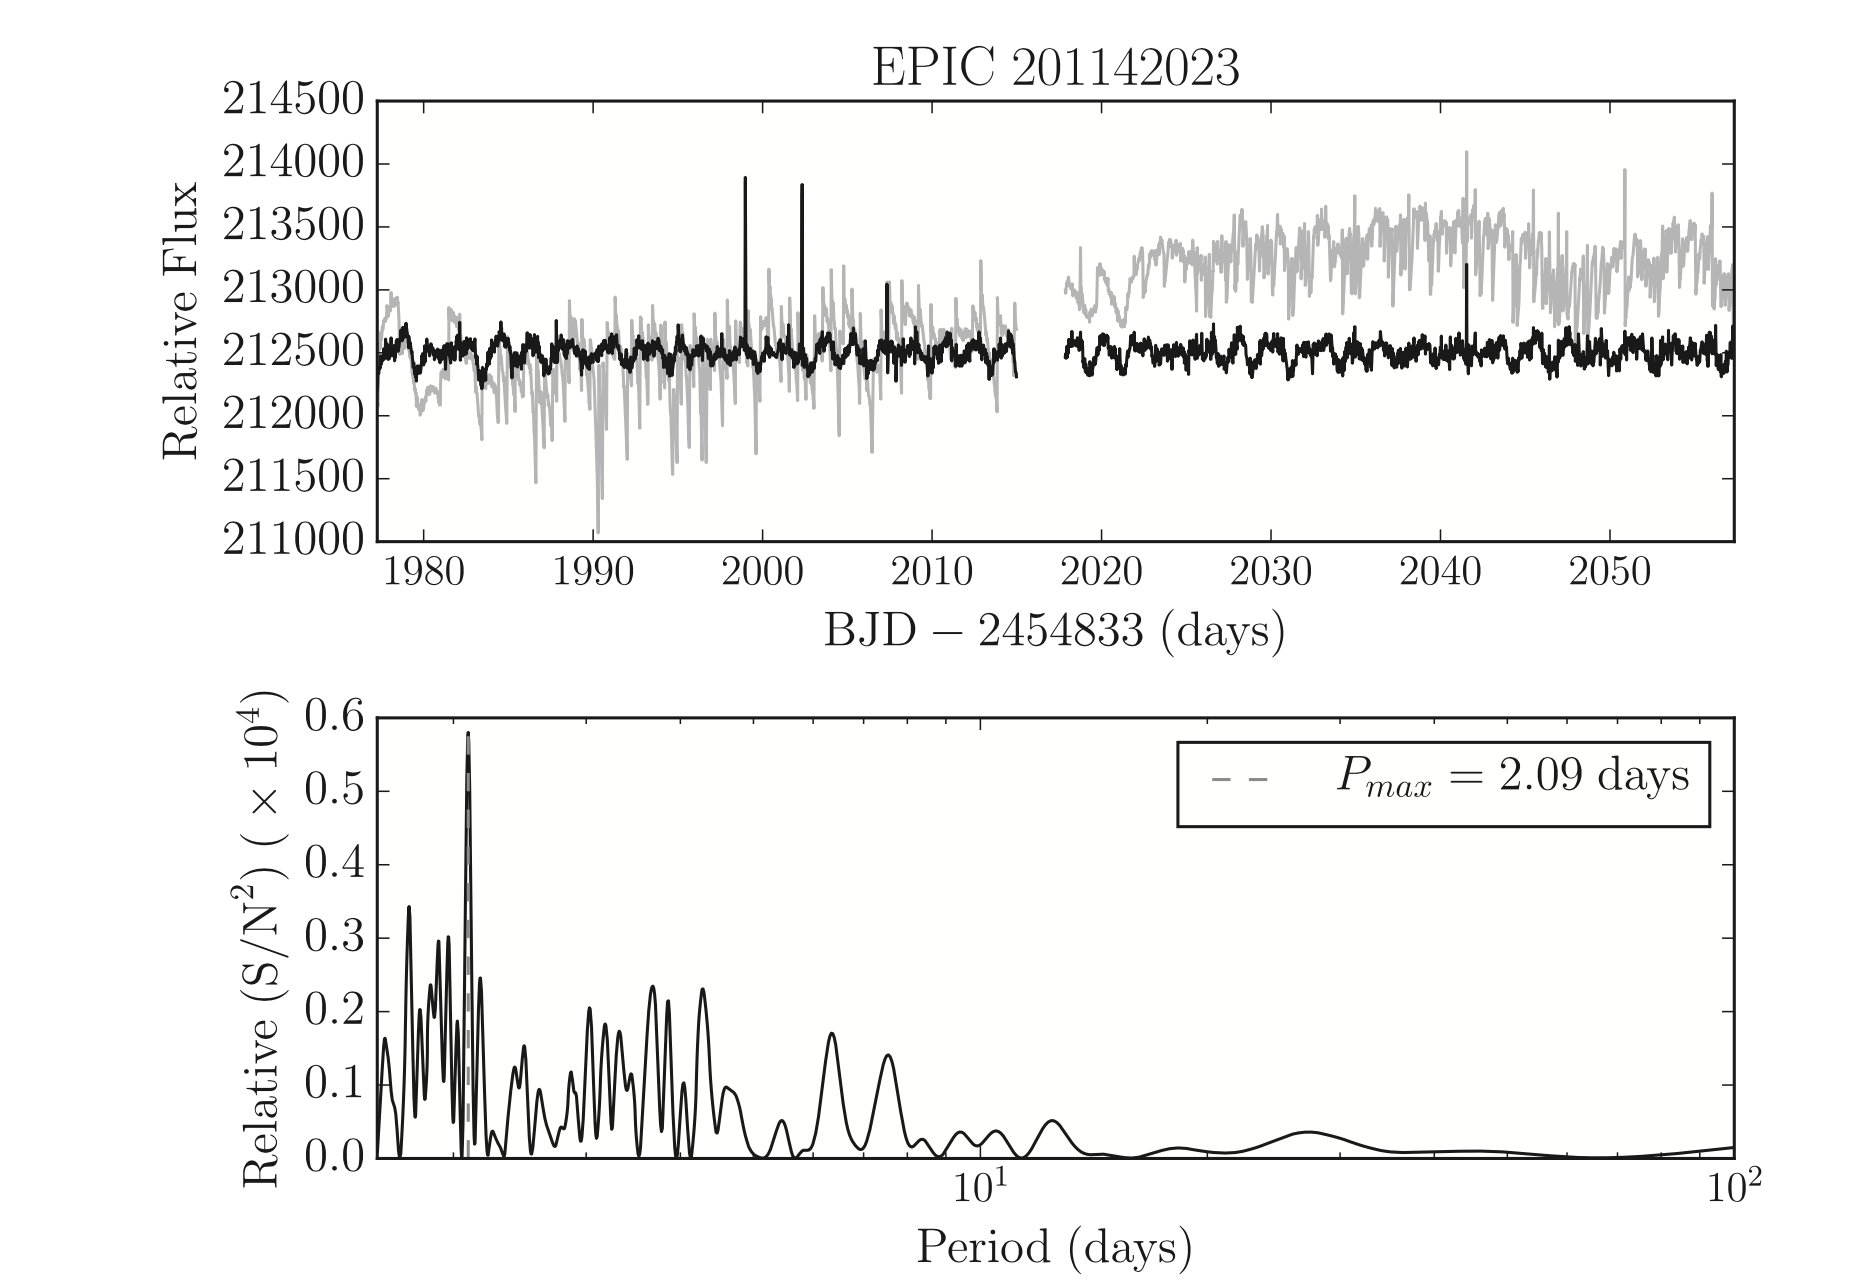
\includegraphics[width=4in]{angus2016_fig6.png}
\caption{
figure 6 from \citet{angus2016}, showing the processing of the light curve and resulting SIPeriodogram. more simple methods give erroneous periods for this object of either 3 days via ACF, or 59 days via normal Lomb-Scargle methods.
}
\label{fig:cmd}
\end{figure}


%%%%%%%%%
\subsection{Mapping Ages in each Field}

%%%%%%%%%
\subsection{Combining with Gaia}


\begin{figure}[!th]
\centering
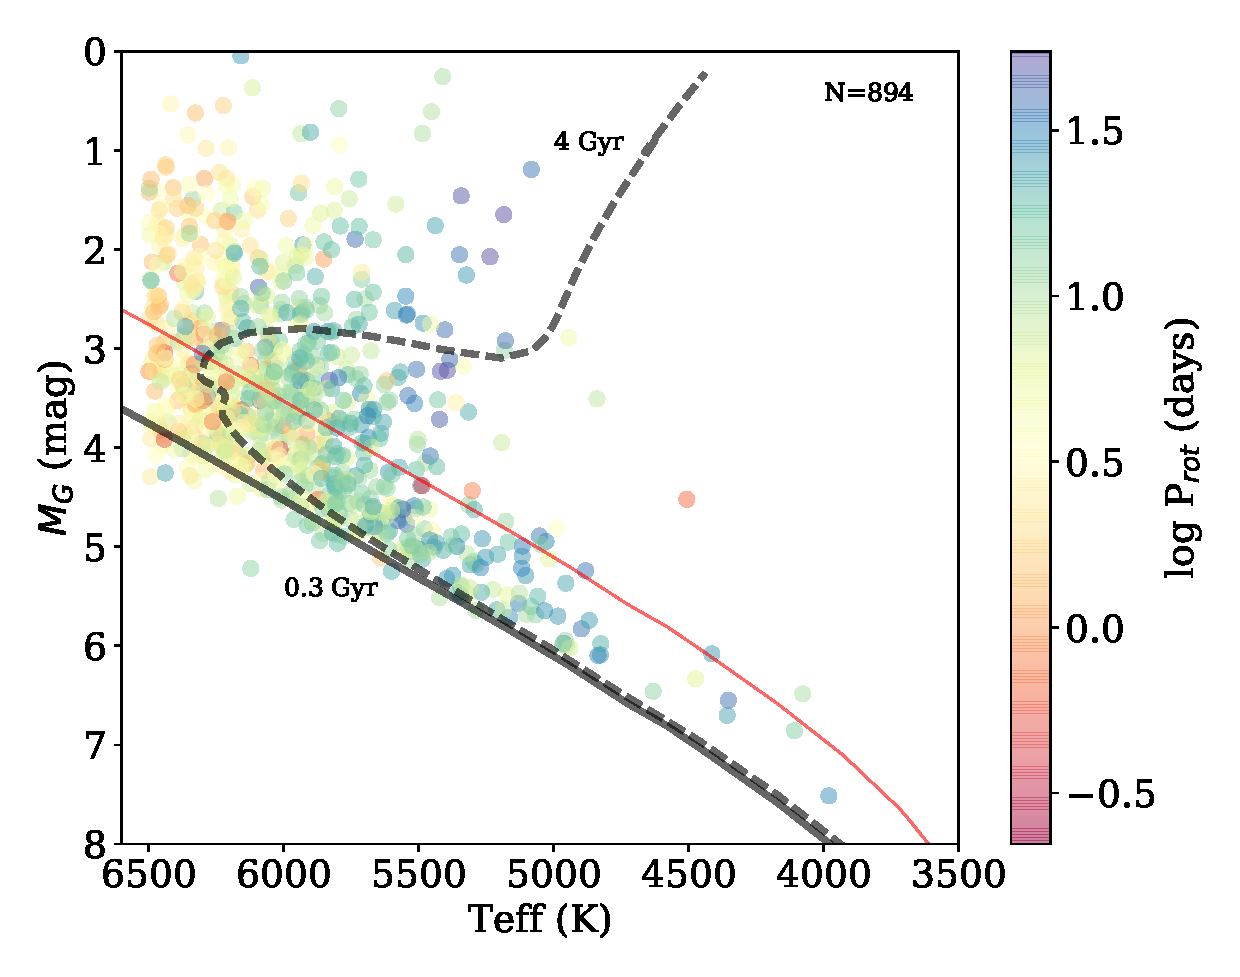
\includegraphics[width=4in]{davenport2016_fig2}
\caption{figure 2 from \citet{davenport2017}, showing temperature from KIC versus absolute magnitude from Gaia}
\label{fig:cmd}
\end{figure}




%%%%%%%%%%%%%%%%%%%
\section{Team Qualifications}
PI Davenport has used \Kepler to conduct the largest survey to-date of stellar activity from flares, as well as multiple investigations of starspots and their evolution with time using \Kepler data. From these studies, Davenport has developed an age model for flare activity that will be directly comparable to the ages and starspot amplitudes derived from this study. He has also recently discovered the rotation period bimodality first noted with \Kepler M dwarfs by \citet{mcquillan2013} extends to G and K dwarf stars \citep{davenport2017}.
Davenport previously collaborated on NASA ADP grant NNX09AC77G to characterize NIR variability using the 2MASS Calibration Scan Point Source Working Database \citep{davenport2012,davenport2015a}.
He has mentored numerous students on projects using \Kepler data, resulting in student-led publications such as the flare activity of a unique M dwarf binary system GJ 1245AB \citep{lurie2015}, and exploring the poorly understood origins of wide binary stars through stellar rotation (R. Clarke in prep). He will manage the overall project, and lead the investigation and publication of the period bimodality exploration. 

Co-I Angus is an expert in the extraction of periodic signals from \Kepler data using Gaussian Processes \citep{angus2016c} and other cutting-edge statistical techniques. She is the author of tools for generating Systematics-Insensitive Periodograms for both \Kepler and K2 data \citep{angus2016}, as well as new gyrochronology calibrations using \Kepler asteroseismic targets \citep{angus2015}. She will lead the effort to measure and publish rotation periods for all K2 sources, and lead the graduate student in measuring ages for field stars.



%%%%%%%%%%%%%%%%%%%
\section{Relevance to NASA Programs}



%%%%%%%%%%%%%%%%%%%
%\section{Relevance to NASA Programs}



\clearpage
%\pagestyle{empty}

\bibliography{/Users/davenpj3/Dropbox/references}


\end{document}

